\documentclass[12pt, a4paper]{article}
\usepackage{CJKutf8}
\usepackage{float}
\usepackage{graphicx}
\date{\today}
\author{李昱伯\footnote{R07522803}、李宜修\footnote{R07522802}、黎純蕙\footnote{R07522840}、林晨涵\footnote{R07522844}}
\title{工業4.0下之軟硬體系統開發\\
期末專題計劃}

\begin{document}
\begin{CJK*}{UTF8}{bkai}
\maketitle

期末專題架構選擇:
\begin{itemize}
  \item 研華寶元 Linux 系列控制器
  \item Wired via LwIP/Wifi via CC3100
  \item noSQL
\end{itemize}

\textbf{實驗架構}
\begin{figure}[H]
  \centering
  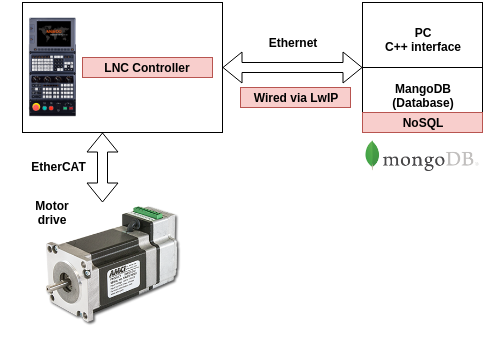
\includegraphics[scale=0.7]{flow4.png}
\end{figure}

\newpage
\textbf{控制器程式流程}
建立控制器連線架構,如下圖:
\begin{figure}[H]
  \centering
  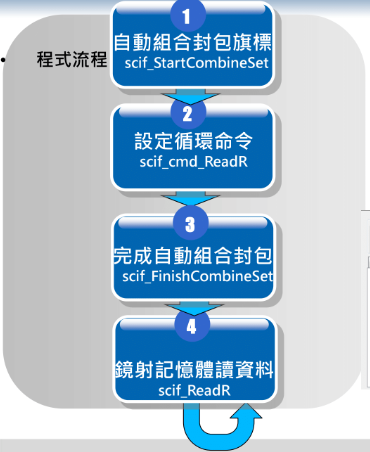
\includegraphics[scale=0.5]{controller.png}
\end{figure}

建立控制器資訊封包,如下圖:
\begin{figure}[H]
  \centering
  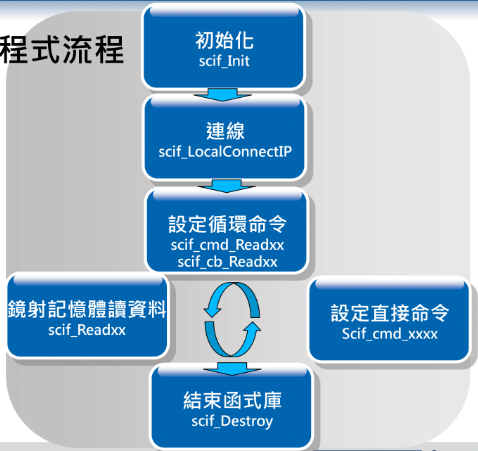
\includegraphics[scale=0.5]{controller2.png}
\end{figure}

分工計劃:
\begin{enumerate}
  \item 控制器資料擷取:李宜修、李昱伯
  \item 資料庫建立:黎純蕙、林晨涵
\end{enumerate}
\end{CJK*}
\end{document}
